\documentclass{article}

\usepackage[final]{style}
\usepackage[utf8]{inputenc} % allow utf-8 input
\usepackage[T1]{fontenc}    % use 8-bit T1 fonts
\usepackage{hyperref}       % hyperlinks
\usepackage{url}            % simple URL typesetting
\usepackage{booktabs}       % professional-quality tables
\usepackage{amsfonts}       % blackboard math symbols
\usepackage{nicefrac}       % compact symbols for 1/2, etc.
\usepackage{microtype}      % microtypography
\usepackage{verbatim}
\usepackage{graphicx}       % for figures

\usepackage{caption}
\usepackage{graphicx, subfig}

\usepackage{amsmath,bm}

\usepackage{mathrsfs}
\usepackage{amssymb}

% Self-defined macros
\newcommand{\matr}[1]{\mathbf{#1}}
\newcommand{\proba}[1]{\mathsf{P}(#1)}
\newcommand{\expect}[1]{\mathsf{E}[#1]}
\newcommand{\var}[1]{\mathsf{Var}(#1)}
\newcommand\defeq{\stackrel{\text{!}}{=}}

\title{Exercise 06 of Machine Learning [IN 2064]}

\author{
  Name: Yiman Li \\
  \textbf{Matr-Nr: 03724352} \\
  cooperate with Kejia Chen(03729686)\\
}

\begin{document}

\maketitle

\section*{Problem 1}
The visualization is shown in Figure \ref{Problem 1}. We can see the set $\bm{\mathcal{X}}$ is convex, so in order to find the maximum, we can just try in 4 different vertices and will find that the maximizer $\bm{\theta}_{max}$ is located at the point $(9, 3)$.\\
In contrast, in order to find the minimizer, we just need to find the maximizer of $-f(\bm{\theta})$. Since $f(\bm{\theta})$is a linear function, then both $f(\bm{\theta})$ and $-f(\bm{\theta})$ are convex functions, so still doing experiments in different vertices in order to find the maximizer of $-f(\bm{\theta})$, which is located at the point $(5, 7)$.
\begin{figure}[htbp]
	\centering
	\begin{minipage}{6.7cm}
		\centering
		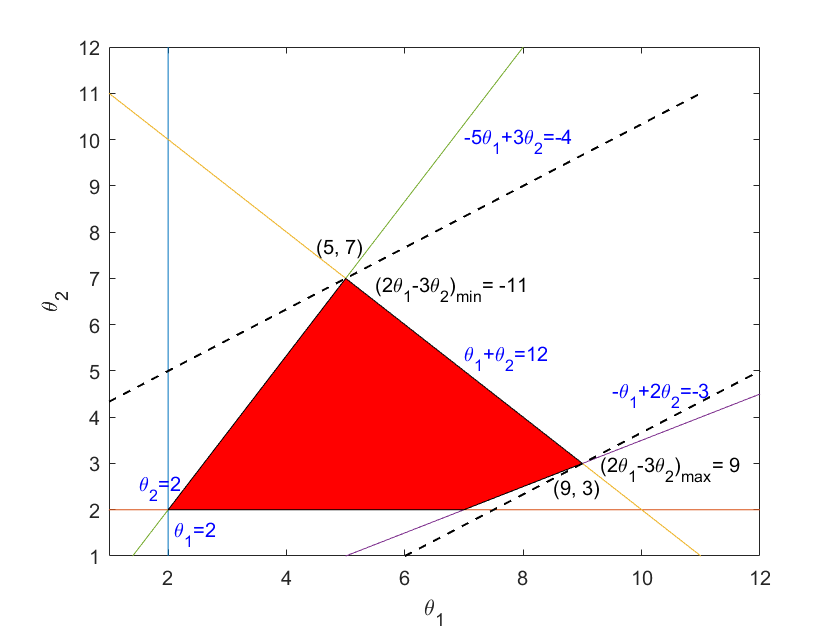
\includegraphics[scale=0.3]{figure1.png}
		\caption{Visulization 1}
		\label{Problem 1}
	\end{minipage}
	\begin{minipage}{6.7cm}
		\centering
		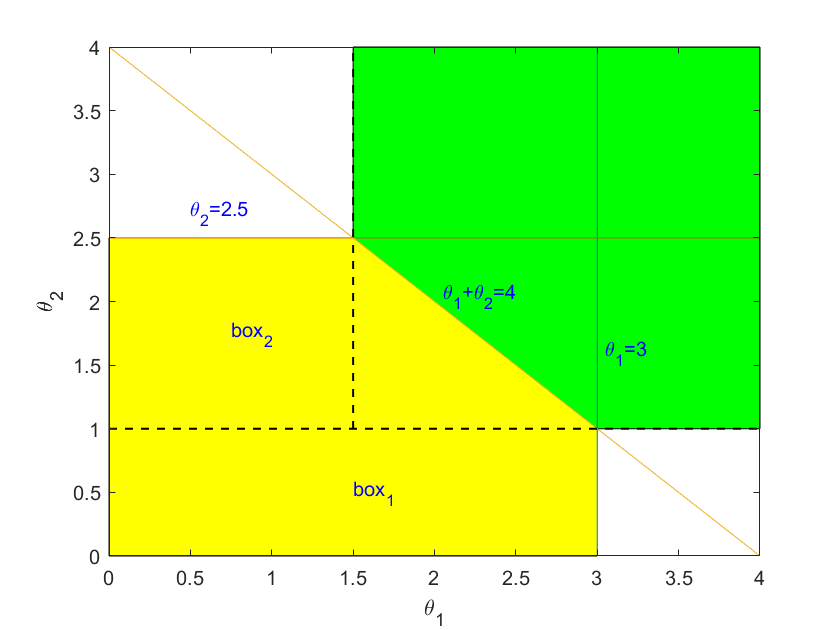
\includegraphics[scale=0.3]{figure2.png}
		\caption{Visulization 2}
		\label{Problem 2}
	\end{minipage}		
\end{figure}
So we have:
\begin{eqnarray}
f(\bm{\theta})_{max} = f(9,3) = 9\\
f(\bm{\theta})_{min} = f(5,7) = -11
\end{eqnarray}
\section*{Problem 2}
a)The Visulization is shown in Figure \ref{Problem 2}. When doing the projection, the points outside the green area are just project onto box, so
\begin{equation}
	(\pi_\mathcal{X}(\bm{p}))_i = min(max(l_i, p_i), u_i)
\end{equation}
But for points $\bm{p}=(x,y)$ in green region, the hyperplane is defined by points $\bm{a}=(1.5, 2.5)$, $\bm{b}=(3,1)$, so we have
\begin{equation}
	\begin{aligned}
		\pi_{\mathcal{X}_{a,b}}(\bm{p})
		&= (1.5, 2.5) + \frac{(x-1.5)\cdot 1.5 + (y-2.5)\cdot -1.5}{4.5}\cdot (1.5, -1.5)\\
		&= (\frac{x-y+4}{2},\frac{y-x+4}{2})
	\end{aligned}
\end{equation}
So in summary, we have the closed form projection for point $\bm{p} = (p_x, p_y)$
\begin{equation}
\pi_\mathcal{X}(\bm{p})=
\begin{cases}
	(min(max(0, 3), p_x),\ min(max(0, 1), p_y)), & \text{if}\ p_y \leq 1;\\
	(x=min(max(0,1.5), p_x),\ y=min(max(1, 2.5), p_y)), & \text{if}\ p_x<1.5, p_y >1;\\
	(\frac{p_x-p_y+4}{2},\frac{p_y-p_x+4}{2}), & \text{if p in region green}. 
\end{cases}
\end{equation}
b)Firstly, the derivative of the function is 
\begin{equation}
	f'(\bm{\theta}) = f'(\theta_1, \theta_2) = (2(\theta_1-2), 4(2\theta_2-7))
\end{equation}

Starting from $\bm{\theta}^{(0)}=(2.5, 1)$, we have
\begin{equation}
	\begin{aligned}
		\bm{\theta}^{(1)}
		&= \bm{\theta}^{(0)} - \tau \cdot f_0'(\theta_1, \theta_2)\\
		&= (2.5, 1) - 0.05 \cdot (1, -20)\\
		&= (2.45, 2)
	\end{aligned}	
\end{equation}
which is out of the feasible region, so we do projection and obtain that
\begin{equation}
	\begin{aligned}
		\bm{\theta}^{(1)}
		&= (\frac{2.45-2+4}{2},\frac{2-2.45+4}{2})\\
		&= (2.225, 1.775)
	\end{aligned}
\end{equation}
Then
\begin{equation}
	\begin{aligned}
		\bm{\theta}^{(2)}
		&= \bm{\theta}^{(1)} - \tau \cdot f_1'(\theta_1, \theta_2)\\
		&= (2.225, 1.775) - 0.05 \cdot (0.45, -13.8)\\
		&= (2.2025, 2.465)
	\end{aligned}	
\end{equation}
which is again not in the feasible areas, so we need to do the projection job, and will find out the true value:
\begin{equation}
	\begin{aligned}
		\bm{\theta}^{(2)}
		&= (\frac{x-y+4}{2},\frac{y-x+4}{2})\\
		&= (1.86875, 2.13125)
	\end{aligned}
\end{equation}

\section*{Problem 3}
Let $\bm{\theta}^*$ be a minimizer of the primal problem and $\bm{\alpha}^*$ a maximizer of the dual problem, then the dual function is given by
\begin{equation}
	\begin{aligned}
		g(\bm{\alpha})
		&= \mathop{\arg\min}_{\theta}\ \ L(\bm{\theta}, \bm{\alpha})\\
		&= \mathop{\arg\min}_{\theta}\ \ (\theta_1 - \sqrt{3}\theta_2) + \alpha(\theta_1^2+\theta_2^2-4)	
	\end{aligned}
\end{equation}
find the minimizing $\bm{\theta}$ from the optimality condition
\begin{equation}
	\nabla_x\ L(\bm{\theta}, \bm{\alpha}) = (2\alpha\theta_1+1) + (2\alpha\theta_2 - \sqrt{3}) = 0
\end{equation}
which yields  $\bm{\theta}^*=(-\frac{1}{2\alpha}, \frac{\sqrt{3}}{2\alpha})$.Therefore the dual function is
\begin{equation}
	\begin{aligned}
		g(\alpha)
		&= (\theta_1 - \sqrt{3}\theta_2) + \alpha(\theta_1^2+\theta_2^2-4)\\
		&= -(\frac{1}{\alpha} + 4\alpha)
	\end{aligned}
\end{equation}
Since $\alpha \geq 0$, so we have $\bm{\alpha}^* = \frac{1}{2}$. Then according to reference \cite{Boyd:2004:CO:993483}, when Slater's condition holds and the primal problem is convex, which is exactly the problem 3's condition, we will have strong duality here. So using $\alpha = \frac{1}{2}$, we get $\bm{\theta}^* = (\theta_1, \theta_2) = (-1, \sqrt{3})$

\section*{Problem 4}
We can rewrite the problem in the following form:
\begin{equation}
	\begin{aligned}
		&\mathrm{minimize}_{\bm{w}, b}\ \ f_0(\bm{w}) = \frac{1}{2}\bm{w}^T\bm{w}\\
		&\text{subject to}\ \ f_i(\bm{w}) = 1 - y_i(\bm{w}^T\bm{x}_i + b) \leq 0
	\end{aligned}
\end{equation}

\begin{itemize}
	\item 
	Firstly, we get the derivatives of the function as below:
	\begin{eqnarray}
	\nabla_{\bm{w}}f_0 = \bm{w}\\
	\nabla_{\bm{w}}^2f_0 = 1
	\end{eqnarray}
	We see the second order derivative is positive, so the object function is convex.\\
	\item Then since all the constraint functions are affine, so their second order derivatives are all 0, and we can say that they are all convex.\\
	\item If the data is linearly separable, there exists a hyperplane to separate the data, so that $\bm{w}^T\bm{x}_i + b \geq 1$ for $y_i=1$, and $\bm{w}^T\bm{x}_i + b \leq -1$ for $y_i=-1$. So there exists a feasible $\bm{w}$ such that all the constraints are satisfied.
\end{itemize}             
Under the 3 conditions mentioned above, the Slater's constraint qualification is fulfilled, so the strong duality holds here.



% References
\small
\bibliographystyle{plain}
\bibliography{bibliography7}
\end{document}
